% =====================================================================
% When does group-conditional conformal calibration help?
% Subgroup coverage, small-group failure, and an uncertainty audit of TabPFN
%
% Target: International Journal of Approximate Reasoning (IJAR, Elsevier)
% =====================================================================
\documentclass[review,12pt]{elsarticle}

\usepackage{amsmath,amssymb,amsfonts}
\usepackage{booktabs}
\usepackage{multirow}
\usepackage{graphicx}
\graphicspath{{figures/}{../figures/}}
\usepackage{xcolor}
\usepackage[hidelinks]{hyperref}
\usepackage{orcidlink}
\usepackage{lineno}
\modulolinenumbers[5]


\journal{International Journal of Approximate Reasoning}

\begin{document}

\begin{frontmatter}

\title{When does group-conditional conformal calibration help? Subgroup coverage, small-group failure, and an uncertainty audit of TabPFN}

\author[inst1]{Nadim Mahmud Dipu\,\orcidlink{0009-0005-8767-1636}}
\ead{nadim.mahmud.dipu@g.bracu.ac.bd}
\affiliation[inst1]{organization={Brac University}, city={Dhaka}, country={Bangladesh}}

\begin{abstract}
Split conformal prediction endows any classifier with finite-sample, distribution-free \emph{marginal} coverage, but marginal validity says nothing about how miscoverage is distributed across protected subgroups. We study when Mondrian (group-conditional) calibration repairs subgroup miscoverage and when it backfires, on three US Census tasks (folktables; California), wrapping multiple predictors in split conformal prediction across three confidence levels and four group taxonomies. At a $90\%$ target the worst-covered age group receives only $86.2\%$ coverage (gap $0.081$) although every model meets the marginal guarantee; Mondrian calibration repairs this (gap $\to 0.051$) at a mean set-size cost of $0.021$, but \emph{increases} the race-axis gap from $0.044$ to $0.057$, where the smallest calibration stratum holds only $\approx\!84$ points. We explain both regimes with an exact finite-sample null model: simulating the Beta--binomial law of realized per-group coverage shows that the age axis carries genuine structural bias (observed marginal gap $0.081$ against $0.032$ under the zero-bias null), whereas the race axis is dominated by sampling noise ($0.044$ against $0.036$), so stratification has little bias to remove and its threshold noise dominates---observed Mondrian gaps match the simulated noise floor on every axis. The diagnostic is computable \emph{before} deployment from $\{\alpha, n_g, |\mathcal{G}|\}$ alone, and these effects are nearly identical across predictors. As the audited model, TabPFN is the most reliable base learner tested: adaptive ECE $0.026$ versus $0.075$/$0.052$ for untuned GBDTs, no measurable benefit from temperature scaling, and the smallest prediction sets. We also caution that non-randomized APS is silently degenerate on binary tasks.
\end{abstract}

\begin{keyword}
conformal prediction \sep equalized coverage \sep Mondrian conformal prediction \sep uncertainty quantification \sep algorithmic fairness \sep TabPFN
\end{keyword}

\end{frontmatter}

\linenumbers

% =====================================================================
\section{Introduction}
\label{sec:intro}

Set-valued prediction with coverage guarantees has become a standard tool for trustworthy machine learning. Given any classifier and an exchangeable calibration sample, split (inductive) conformal prediction returns a prediction set that contains the true label with a user-specified probability $1-\alpha$, distribution-free and in finite samples \cite{vovk2005,papadopoulos2002,shafer2008,angelopoulos2023,fontana2023}. This guarantee, however, is \emph{marginal}: it averages over the whole population. In the high-stakes tabular settings where conformal prediction is increasingly deployed---credit scoring, benefits eligibility, clinical triage---algorithmic disparities have repeatedly been documented at the subgroup level \cite{obermeyer2019,chouldechova2017}, and decisions concern individuals who belong to protected demographic groups, and a guarantee that holds on average can fail conditionally. A $90\%$ marginal guarantee is compatible with, say, $86\%$ coverage for one group and $94\%$ for another, silently concentrating error on the worse-covered group \cite{romano2020eq}. Exact conditional coverage is provably unattainable without distributional assumptions \cite{vovk2012,barber2021limits}, so the practical question is not whether the gap between marginal and conditional validity exists---it must---but how large it is on real group structures, and what can be done about it.

The textbook remedy is \emph{Mondrian} (group-conditional) conformal prediction \cite{vovk2003,vovk2012,romano2020eq}, which calibrates a separate quantile within each group and so guarantees coverage \emph{within} every group---``equalized coverage''---rather than only on average. That guarantee holds in expectation over calibration draws, and it is purchased with data: each group's threshold is estimated from only the $n_g$ calibration points falling in that group. When some groups are small---as protected attributes with imbalanced categories routinely are---those thresholds are noisy, and the realized per-group coverage can vary enough that group-conditional calibration \emph{increases} the empirical disparity it was meant to remove. The practically important question is therefore when Mondrian stratification helps versus harms in finite samples, and how a practitioner should decide \emph{in advance}. We answer it with an exact, simulable finite-sample null model: because the conditional coverage of a split conformal predictor follows a known Beta law \cite{vovk2012,angelopoulos2023}, the entire distribution of the realized per-group coverage gap \emph{under zero structural bias} can be computed from the target level $\alpha$, the per-group calibration counts $\{n_g\}$, and the test stratum sizes alone---before any group-conditional calibration is run. Comparing the observed marginal gap to this null tells the practitioner whether there is bias to repair; comparing it to the Mondrian null tells them what gap stratification would leave behind.

We situate this study in the tabular regime and pair it with a second, timely question: which base learner to trust. For over a decade gradient-boosted decision trees (GBDTs) have been the default for tabular classification \cite{grinsztajn2022}, but they are now challenged by \emph{tabular foundation models}, most prominently TabPFN, a prior-data fitted network (PFN) that performs supervised learning as a single forward pass of in-context inference \cite{tabpfn2023,tabpfn2025}. The choice of base learner still matters for uncertainty: the conformal quantile step repairs \emph{validity} for any model, but the calibration of the underlying probabilities controls set \emph{efficiency}. TabPFN's developers report favourable calibration \cite{tabpfn2025}, but we are aware of no audit that places a tabular foundation model inside a split conformal pipeline under a protocol matched to strong baselines, nor one that examines the per-group coverage its scores induce. We therefore adopt TabPFN as the model under audit---against XGBoost, LightGBM, and an MLP---while emphasizing that the conformal-fairness findings turn out not to depend on the model at all.

We study three binary prediction tasks derived from US Census microdata via the folktables package \cite{ding2021}---ACSIncome, ACSEmployment, and ACSPublicCoverage for California---each carrying protected attributes (sex, race, age). We compare the models under an identical train/calibration/test protocol with five random seeds, wrapping every model in split conformal prediction at three target levels ($80\%$, $90\%$, $95\%$) with the LAC score, in both marginal and Mondrian variants, across four group taxonomies. Our research questions and headline answers are:

\begin{itemize}
  \item \textbf{RQ1 (Calibration).} \emph{Are TabPFN's native probabilities better calibrated than those of GBDTs and an MLP under a matched protocol?} Against untuned GBDTs, yes: pooled adaptive ECE is $0.026$ for TabPFN versus $0.075$ (XGBoost) and $0.052$ (LightGBM), with paired Wilcoxon $p<10^{-4}$; TabPFN is statistically indistinguishable from the MLP while being more accurate, and temperature scaling adds no significant improvement. Against temperature-scaled GBDTs---the recipe practitioners actually deploy---the calibration gap closes (all three reach adaptive ECE $0.026$), but TabPFN retains a significant edge on the proper scoring rules (Brier and NLL, $p=6.1\times10^{-5}$) and on accuracy.
  \item \textbf{RQ2 (Conformal validity and efficiency).} \emph{Do all models achieve nominal marginal coverage, and which yields the most efficient prediction sets?} With the LAC score, empirical coverage tracks all three targets to within one percentage point for every model; TabPFN yields the smallest sets at every level (e.g., $1.296$ vs.\ $1.327$--$1.363$ at $90\%$; $p<10^{-3}$ against each baseline). We also document, as a practical caution, that APS \emph{without randomization} is degenerate on these binary tasks, and report randomized APS for comparison (valid but less efficient than LAC---mean set size $1.409$ vs.\ $1.331$ at the $90\%$ target; Section~\ref{sec:rq2}).
  \item \textbf{RQ3 (Coverage fairness).} \emph{Does marginal conformal prediction hide subgroup miscoverage, and does Mondrian conformal repair it?} Marginal coverage conceals an age-related gap of $0.081$ at the $90\%$ target (worst-group coverage $0.862$). Mondrian stratification repairs this on the age axis (gap $\to 0.051$) at a small efficiency cost, is neutral on the already-equitable sex axis, but \emph{increases} the empirical gap on the race axis (from $0.044$ to $0.057$) without improving worst-group coverage. The exact null model of Section~\ref{sec:theory} explains all three outcomes quantitatively, and the effects are nearly identical across all predictors: coverage fairness is governed by the conformal procedure and the group structure, not by the model.
\end{itemize}

\noindent Our contributions are: (1) a controlled empirical demonstration, across multiple predictors and three census tasks, that marginal conformal validity conceals systematic subgroup miscoverage, including a documented regime in which group-conditional (Mondrian) calibration \emph{worsens} the realized disparity; (2) an exact, simulable finite-sample null model for the per-group coverage gap---built on the Beta law of split-conformal coverage and a binomial test-measurement layer---together with a closed-form approximation, which decomposes any observed gap into structural bias and sampling noise and yields an \emph{a priori} test of whether Mondrian stratification can help on a given axis; (3) a matched-protocol audit of TabPFN's calibration and conformal efficiency against GBDT and MLP baselines, within a conformal and group-conditional pipeline that prior TabPFN evaluations \cite{tabpfn2025,mcelfresh2023} do not cover; (4) support-aware deployment guidance derived from the null model; and (5) an open, fully scripted pipeline with committed per-seed result files, the null-model simulator, and a verification script that recomputes every reported number.

The remainder of the paper is organized as follows. Section~\ref{sec:related} reviews related work. Section~\ref{sec:background} recalls the calibration metrics, split conformal prediction, the LAC and APS scores, and Mondrian conformal prediction. Section~\ref{sec:theory} develops the finite-sample null model, validates it by exact simulation, and derives the closed-form floor. Section~\ref{sec:method} details datasets, models, protocol, and the statistical analysis plan. Section~\ref{sec:results} reports results for RQ1--RQ3 and reads the empirical gaps against the simulated null. Section~\ref{sec:discussion} derives deployment guidance, Section~\ref{sec:limitations} discusses threats to validity, and Section~\ref{sec:conclusion} concludes.

% =====================================================================
\section{Related work}
\label{sec:related}

\paragraph{Conformal prediction and conditional validity.}
Split (inductive) conformal prediction converts any scoring model into set-valued predictions with finite-sample, distribution-free marginal coverage under exchangeability \cite{vovk2005,papadopoulos2002,shafer2008,lei2018,angelopoulos2023}; comprehensive reviews are given by Fontana et al.\ \cite{fontana2023} and Angelopoulos and Bates \cite{angelopoulos2023}. The framework extends well beyond the split-classification setting we study: conformalized quantile regression \cite{romano2019cqr}, jackknife+ aggregation \cite{barber2021jackknife}, localized weighting \cite{guan2023}, risk-controlling generalizations of coverage \cite{bates2021}, and end-to-end training of the score function \cite{stutz2022}. Vovk \cite{vovk2012} systematized the stronger notions of conditional validity (training-, object-, and label-conditional) and showed how Mondrian taxonomies achieve category-wise validity at a finite-sample cost; the training-conditional behaviour of split conformal prediction---the Beta law we build on in Section~\ref{sec:theory}---is analyzed in \cite{vovk2012,bian2023}. Barber et al.\ \cite{barber2021limits} proved that exact object-conditional coverage is impossible without distributional assumptions, delimiting what any procedure can promise. For classification, Lei \cite{lei2014} studied set-valued classifiers with confidence; the LAC/homogeneous score thresholds $1-\hat p_y$ \cite{sadinle2019}, while APS accumulates sorted class probabilities to improve conditional coverage \cite{romano2020aps}, with regularized variants for many-class problems \cite{angelopoulos2021} and quantile-regression-based alternatives targeting conditional validity \cite{cauchois2021}. APS requires tie-breaking randomization for exact validity, a detail our results show to be decisive on binary tasks.

\paragraph{Group-conditional coverage and fairness in uncertainty quantification.}
The algorithmic-fairness literature has produced a family of group-level criteria for point predictions---demographic parity and disparate impact \cite{dwork2012,feldman2015}, equalized odds and opportunity \cite{hardt2016}---together with impossibility results showing that calibration-style and error-rate-style criteria cannot in general be satisfied simultaneously \cite{kleinberg2017,chouldechova2017,pleiss2017}; see \cite{mehrabi2021,barocas2023} for surveys. \emph{Equalized coverage} transports this program to set-valued prediction: it asks that prediction sets cover each protected group at the nominal rate, achievable by Mondrian/group-conditional calibration \cite{romano2020eq,vovk2003,vovk2012}. Subsequent work studies class- and group-conditional validity, its finite-sample costs, and approximate or multivalid conditional coverage at controlled cost \cite{ding2023,gibbs2023,jung2023}; multicalibration pursues the analogous goal for probability estimates over rich collections of subpopulations \cite{hebert2018}, and Cherian and Cand{\`e}s \cite{cherian2024} develop inferential tools for auditing group-level performance disparities of a fixed model. Empirically, Lu et al.\ \cite{lu2022fair} audit per-group coverage of conformal predictors in medical imaging and apply equalized coverage across skin-tone subgroups, and the Mondrian literature has long observed that thresholds in sparse categories are noisy, motivating bias-reduction schemes for small strata \cite{lofstrom2015}. Our contribution to this line is not the observation that small groups are problematic---that is implicit in the guarantee's $1/(n_g+1)$ slack and explicit in \cite{vovk2012,lofstrom2015}---but an \emph{exact, pre-deployment null model} for the realized max--min gap statistic that practitioners actually report, a controlled demonstration that plain Mondrian calibration can \emph{increase} that statistic relative to marginal calibration on a real protected attribute, and a decomposition of observed gaps into structural bias and sampling noise. To our knowledge no prior audit places a tabular foundation model in this pipeline, and the marginal-versus-Mondrian crossover as a function of calibration support has not previously been isolated and predicted in advance; we position our novelty on exactly those two points rather than claiming the broader intersection is unoccupied.

\paragraph{Calibration of machine-learning classifiers.}
Probability calibration has a long history rooted in forecast verification and proper scoring rules \cite{brier1950,gneiting2007}. Classical post-hoc recalibration maps for margin classifiers and trees include Platt scaling and isotonic-style transformations \cite{platt1999,zadrozny2002}; boosted trees in particular push scores away from the extremes, motivating such corrections \cite{niculescu2005}. Modern neural networks are frequently miscalibrated and benefit from temperature scaling \cite{guo2017}, with richer multi-class maps such as Dirichlet calibration \cite{kull2019}; calibration further degrades under dataset shift \cite{ovadia2019}, a regime we leave to future work. Metric estimation itself is delicate: binned ECE is biased and binning choices materially affect conclusions \cite{naeini2015,vaicenavicius2019}, and adaptive (equal-mass) binning is the recommended estimator \cite{nixon2019}. We adopt adaptive ECE as our primary metric and report Brier score and NLL as proper-scoring complements \cite{brier1950,gneiting2007}.

\paragraph{Tabular foundation models and prior-data fitted networks.}
For over two decades, ensembles of decision trees---random forests \cite{breiman2001} and gradient boosting \cite{friedman2001}, in the modern implementations XGBoost \cite{chen2016}, LightGBM \cite{ke2017}, and CatBoost \cite{prokhorenkova2018}---have set the bar for tabular prediction, and systematic comparisons repeatedly find them at or near the top against deep alternatives \cite{grinsztajn2022,shwartz2022,borisov2024}, although well-tuned simple networks can be competitive \cite{kadra2021,gorishniy2021}. Foundation-model approaches to tabular data have recently been argued to deserve concerted research attention \cite{vanbreugel2024}. PFNs meta-train a transformer on synthetic datasets drawn from a prior over data-generating mechanisms, so that supervised prediction on a new table reduces to in-context inference \cite{pfn2022}. TabPFN instantiated this idea for small tabular classification \cite{tabpfn2023} and its successor scaled it to larger tables and regression, reporting favourable calibration relative to baselines \cite{tabpfn2025}. Broader evaluations of tabular models have focused on accuracy and AUC \cite{grinsztajn2022,mcelfresh2023}; what remains unexamined, and what we supply, is how a PFN's probabilities behave as conformity scores inside a split conformal pipeline---validity, efficiency, and per-group coverage---under a protocol matched to GBDT and MLP baselines.

\paragraph{Benchmarking tabular deep learning under matched protocols.}
A recurring lesson of tabular benchmarking is that conclusions are protocol-sensitive---tuning budgets, preprocessing, and split design can reverse rankings \cite{grinsztajn2022,gorishniy2021,kadra2021}---and that cross-dataset model comparisons require care in the choice of statistical machinery \cite{demsar2006}. We therefore hold the entire pipeline fixed across models and vary only the predictor, and we scope all model-comparison claims to the out-of-the-box configurations we test (Section~\ref{sec:limitations}).

% =====================================================================
\section{Background and preliminaries}
\label{sec:background}

We consider classification with covariates $X \in \mathcal{X}$, labels $Y \in \mathcal{Y} = \{1,\dots,K\}$ (here $K=2$), and, for fairness analyses, a protected attribute $A \in \mathcal{A}$. A probabilistic classifier outputs $\hat p(y \mid x)$.

\subsection{Calibration metrics}
A classifier is \emph{top-label calibrated} if $\Pr\!\big(Y = \hat y \,\big|\, \hat p(\hat y \mid X) = c\big) = c$ for all confidence levels $c$, where $\hat y = \arg\max_y \hat p(y\mid x)$. The expected calibration error \cite{naeini2015} partitions test predictions into $B$ bins $\{\mathcal{B}_b\}$ by confidence and computes
\begin{equation}
\mathrm{ECE} \;=\; \sum_{b=1}^{B} \frac{|\mathcal{B}_b|}{n} \,\Big|\, \mathrm{acc}(\mathcal{B}_b) - \mathrm{conf}(\mathcal{B}_b) \,\Big| ,
\label{eq:ece}
\end{equation}
where $\mathrm{acc}$ and $\mathrm{conf}$ are the mean accuracy and mean confidence within a bin. We use \emph{adaptive} (equal-mass) binning with $B = 15$ bins as the primary estimator \cite{nixon2019,vaicenavicius2019}; we additionally report the maximum calibration error (MCE), the Brier score $\frac1n\sum_i \|\hat p(\cdot\mid x_i) - e_{y_i}\|_2^2$ \cite{brier1950}, and the negative log-likelihood (NLL), both strictly proper scoring rules \cite{gneiting2007}. \emph{Temperature scaling} \cite{guo2017}---the simplest member of the post-hoc recalibration family that includes Platt scaling and multiclass extensions \cite{platt1999,zadrozny2002,kull2019}---post-processes logits $z$ as $\mathrm{softmax}(z/T)$ with a single scalar $T>0$ fit by NLL minimization; it is monotone and therefore accuracy-preserving.

\subsection{Split conformal prediction and the Beta law of its coverage}
\label{sec:splitcp}
Split conformal prediction \cite{papadopoulos2002,vovk2005,shafer2008} uses a held-out calibration set $\{(x_i, y_i)\}_{i=1}^{n}$, disjoint from training data, and a conformity score $s(x,y)$ measuring how poorly $y$ conforms at $x$ (larger $=$ worse). Let
\begin{equation}
\hat q \;=\; \text{the } \frac{\lceil (n+1)(1-\alpha) \rceil}{n}\text{-th empirical quantile of } \{s(x_i,y_i)\}_{i=1}^{n}.
\label{eq:quantile}
\end{equation}
The prediction set for a test point $x$ is $C(x) = \{\, y : s(x,y) \le \hat q \,\}$. If the calibration and test points are exchangeable, then for any score function and any model,
\begin{equation}
1-\alpha \;\le\; \Pr\big(Y_{\mathrm{test}} \in C(X_{\mathrm{test}})\big) \;\le\; 1-\alpha + \frac{1}{n+1},
\label{eq:coverage}
\end{equation}
where the upper bound holds when scores are almost surely distinct \cite{lei2018,angelopoulos2023}. Two finer facts matter for this paper. First, coverage in Eq.~\eqref{eq:coverage} is \emph{marginal} over both the test point and the calibration draw; conditional on a particular calibration set, the true conditional coverage is random. With $k = \lceil (n+1)(1-\alpha) \rceil$ and continuously distributed scores, that conditional coverage follows the exact law
\begin{equation}
C \;\sim\; \mathrm{Beta}\big(k,\; n+1-k\big),
\label{eq:beta}
\end{equation}
with mean $k/(n+1) \ge 1-\alpha$ and standard deviation $\approx \sqrt{\alpha(1-\alpha)/n}$ \cite{vovk2012,angelopoulos2023,bian2023}. Second, coverage \emph{measured} on a finite test sample of size $m$ adds a binomial layer: the empirical coverage is $\mathrm{Bin}(m, C)/m$. Both layers are needed to predict what an auditor will actually observe; Section~\ref{sec:theory} builds on exactly this. Exchangeability holds by construction in our protocol---calibration and test points are an i.i.d.\ split of a single dataset---so any subgroup miscoverage we observe is a property of the conditional behaviour the marginal bound leaves unconstrained, not a violation of the bound itself.

\subsection{Conformity scores: LAC and APS}
We evaluate two standard classification scores.
\emph{LAC} (least ambiguous set-valued classifier) \cite{sadinle2019} sets
\begin{equation}
s_{\mathrm{LAC}}(x,y) \;=\; 1 - \hat p(y \mid x),
\end{equation}
which yields the smallest average set size among procedures with marginal validity when probabilities are correct, but offers no conditional-coverage adaptivity. Note that LAC sets can be \emph{empty} when $\max_y \hat p(y\mid x) < 1-\hat q$; we report empty-set rates in Section~\ref{sec:rq2}.
\emph{APS} (adaptive prediction sets) \cite{romano2020aps} sorts classes by predicted probability, $\hat p_{(1)} \ge \dots \ge \hat p_{(K)}$, and scores
\begin{equation}
s_{\mathrm{APS}}(x,y) \;=\; \sum_{j : \hat p_{(j)} > \hat p(y\mid x)} \hat p_{(j)} \;+\; u \cdot \hat p(y \mid x),
\qquad u \sim \mathrm{Unif}(0,1),
\label{eq:aps}
\end{equation}
where the randomization term $u$ is essential for exact validity. The deterministic variant replaces $u$ by $1$, i.e.\ includes the full mass of the label's own class, and is conservative; Section~\ref{sec:rq2} shows this is not a cosmetic detail on binary tasks.

\subsection{Mondrian (group-conditional) conformal prediction and equalized coverage}
Given a partition of the population by a taxonomy $g(x,a) \in \mathcal{G}$ (here: the protected attribute, or the predicted class), Mondrian conformal prediction \cite{vovk2003,vovk2012} computes the quantile in Eq.~\eqref{eq:quantile} \emph{separately within each group}, using the $n_g$ calibration points of group $g$. This yields the group-conditional guarantee
\begin{equation}
\Pr\big(Y \in C(X) \,\big|\, g(X,A) = g\big) \;\ge\; 1-\alpha \qquad \text{for every } g \in \mathcal{G},
\label{eq:mondrian}
\end{equation}
i.e., \emph{equalized coverage} in expectation \cite{romano2020eq}. The price is statistical: each group's threshold $\hat q_g$ is estimated from only $n_g \ll n$ calibration points, so by Eq.~\eqref{eq:beta} the conditional per-group coverage fluctuates about the nominal level with standard deviation $\approx \sqrt{\alpha(1-\alpha)/n_g}$, and the guarantee's finite-sample slack $1/(n_g+1)$ grows as groups shrink. Equalized coverage \emph{in expectation} is thus fully compatible with a \emph{larger realized} disparity than marginal calibration produces when strata are small. Whether that happens on a given axis is precisely what the next section makes computable.

\subsection{Fairness metrics for prediction sets}
For groups $g \in \mathcal{G}$ with empirical per-group coverage $\hat c_g$ and mean set size $\bar k_g$ on the test set, we report the \emph{coverage gap} $\max_g \hat c_g - \min_g \hat c_g$, the \emph{worst-group coverage} $\min_g \hat c_g$, and the \emph{set-size disparity} $\max_g \bar k_g - \min_g \bar k_g$. The max--min gap is the statistic practitioners most often quote, but it is group-count sensitive and anonymous; we therefore treat worst-group coverage as the decision-relevant summary, report named per-group coverages (Table~\ref{tab:pergroup}), and---crucially---always read the gap against its finite-sample null distribution (Section~\ref{sec:theory}) rather than against zero.

% =====================================================================
\section{A finite-sample null model for the per-group coverage gap}
\label{sec:theory}

This section is the conceptual core of the paper. We ask: \emph{what coverage gap should an auditor expect to observe even when there is nothing wrong?} Answering this requires no experimental data---only $\alpha$, the per-group calibration counts $\{n_g\}$, the test stratum sizes $\{m_g\}$, and the exact distributional facts of Section~\ref{sec:splitcp}---and it converts the marginal-versus-Mondrian decision into a computation that can be performed before deployment.

\subsection{Bias and noise: a decomposition of the realized gap}
\label{sec:decomp}
Write the per-group empirical test coverage as $\hat c_g$. Under \emph{marginal} calibration all groups share the single global threshold $\hat q$, so
\begin{equation}
\hat c_g \;\approx\; (1-\alpha) \;+\; b_g \;+\; \varepsilon_g ,
\end{equation}
where $b_g$ is a \emph{structural bias}---the systematic over- or under-coverage the global threshold inflicts on group $g$ because that group's score distribution departs from the pooled one---and $\varepsilon_g$ is sampling noise. The noise term has two sources that must not be conflated: (i) the calibration draw, which perturbs the shared threshold (small, of order $\sqrt{\alpha(1-\alpha)/n}$, and common to all groups), and (ii) \emph{test-side measurement noise}, $\mathrm{sd}(\varepsilon_g) \approx \sqrt{c(1-c)/m_g}$ for a test stratum of size $m_g$, which is \emph{not} small when test strata are small. A race stratum measured on $m_g \approx 100$ test points carries measurement noise of standard deviation $\approx 0.03$ at the $90\%$ level---of the same order as the entire gaps we will report. Consequently the observed marginal gap is \emph{not} a clean estimate of the bias spread $\max_g b_g - \min_g b_g$; it is bias spread plus noise, and on axes with small test strata it can be dominated by the latter.

Under \emph{Mondrian} calibration each group receives its own threshold $\hat q_g$. This removes the bias ($\mathbb{E}[\hat c_g] \ge 1-\alpha$ for every group) but replaces the shared-threshold noise by per-group threshold noise of order $\sqrt{\alpha(1-\alpha)/n_g}$ (Eq.~\eqref{eq:beta}), on top of the same test-side measurement noise. Mondrian thus trades a \emph{bias-driven} gap for a \emph{noise-driven} one, and it can only help when there is more bias to remove than noise to inject.

\subsection{The exact null, by simulation}
\label{sec:mcnull}
Both regimes admit an exact zero-bias null that is trivial to simulate, because every ingredient has a known law:
\begin{itemize}
  \item \textbf{Mondrian null.} For each group $g$, draw the conditional coverage $C_g \sim \mathrm{Beta}(k_g,\, n_g+1-k_g)$ with $k_g = \lceil (n_g+1)(1-\alpha) \rceil$ (thresholds in disjoint strata are independent), then draw the measured coverage $\hat c_g \sim \mathrm{Bin}(m_g, C_g)/m_g$, and record $\max_g \hat c_g - \min_g \hat c_g$.
  \item \textbf{Zero-bias marginal null.} Draw a single shared $C \sim \mathrm{Beta}(k,\, n+1-k)$ from the pooled calibration size $n = \sum_g n_g$, then $\hat c_g \sim \mathrm{Bin}(m_g, C)/m_g$ independently per group. This is the gap an auditor observes under marginal calibration \emph{when all structural biases are zero}---pure measurement noise.
\end{itemize}
The simulation costs seconds (script \texttt{mc\_noise\_floor.py}, committed; $200{,}000$ replicates). Table~\ref{tab:mcnull} reports the resulting expected gaps for the exact group structures of our three protected axes (calibration counts of Table~\ref{tab:groupsizes}; test strata scaled by the $2{,}400/2{,}000$ test-to-calibration ratio), averaged over the three datasets, at all three target levels. Figure~\ref{fig:mcnull} shows the Mondrian null as a function of the smallest stratum for several group counts, with the closed-form approximation of Section~\ref{sec:floor} overlaid.

\begin{table}[t]
\centering
\caption{Simulated zero-bias null expectations of the max--min coverage gap (200{,}000 replicates of the exact Beta--binomial law; group structures from Table~\ref{tab:groupsizes}, averaged over the three datasets), alongside the observed pooled gaps from Section~\ref{sec:rq3}. Reading: an observed gap close to its null is explained by sampling noise; an excess over the null estimates the structural-bias contribution. Per-realization Monte Carlo standard deviations are $0.007$--$0.027$ (largest on race); standard errors of the simulated means are negligible.}
\label{tab:mcnull}
\small
\begin{tabular}{llcccc}
\toprule
 & & \multicolumn{2}{c}{Marginal} & \multicolumn{2}{c}{Mondrian} \\
\cmidrule(lr){3-4}\cmidrule(lr){5-6}
Target & Axis & Null & Observed & Null & Observed \\
\midrule
\multirow{3}{*}{$80\%$} & Sex  & $0.013$ & $0.029$ & $0.019$ & $0.020$ \\
                        & Age  & $0.043$ & $0.151$ & $0.063$ & $0.105$ \\
                        & Race & $0.048$ & $0.057$ & $0.070$ & $0.058$ \\
\midrule
\multirow{3}{*}{$90\%$} & Sex  & $0.010$ & $0.012$ & $0.014$ & $0.013$ \\
                        & Age  & $0.032$ & $0.081$ & $0.047$ & $0.051$ \\
                        & Race & $0.036$ & $0.044$ & $0.052$ & $0.057$ \\
\midrule
\multirow{3}{*}{$95\%$} & Sex  & $0.007$ & $0.012$ & $0.010$ & $0.010$ \\
                        & Age  & $0.023$ & $0.045$ & $0.034$ & $0.037$ \\
                        & Race & $0.026$ & $0.033$ & $0.037$ & $0.038$ \\
\bottomrule
\end{tabular}
\end{table}

\begin{figure}[t]
\centering
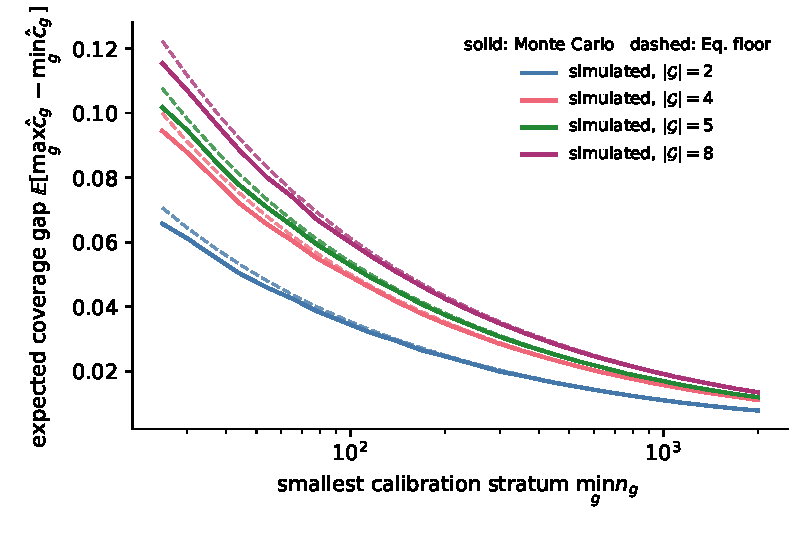
\includegraphics[width=0.72\linewidth]{mc_noise_floor}
\caption{Expected Mondrian coverage gap under the zero-bias null (solid: exact Beta--binomial Monte Carlo; dashed: closed-form approximation, Eq.~\eqref{eq:gapfloor}) as a function of the smallest calibration stratum, for taxonomies with $|\mathcal{G}| \in \{2,4,5,8\}$ groups (one small stratum, remaining strata six times larger; $\alpha=0.1$). The closed form tracks the exact null closely in this one-dominant-stratum regime; for taxonomies with several comparably small strata it underestimates the null (see text), and the simulation should be preferred.}
\label{fig:mcnull}
\end{figure}

\subsection{A closed-form approximation}
\label{sec:floor}
A back-of-envelope version of the Mondrian null is sometimes convenient. Approximating each group's fluctuation as Gaussian with standard deviation $\sigma_g \approx \sqrt{\alpha(1-\alpha)/n_g}$ (Eq.~\eqref{eq:beta}; test-side noise enlarges this further), treating groups as independent, and using the expected range of $|\mathcal{G}|$ such variables, dominated by the noisiest (smallest) stratum,
\begin{equation}
\mathrm{gap}^{\mathrm{Mond}}_{\mathrm{null}} \;\approx\; \sqrt{\frac{\alpha(1-\alpha)}{\min_g n_g}}\,\sqrt{2\ln|\mathcal{G}|}.
\label{eq:gapfloor}
\end{equation}
On our axes this evaluates to $0.011$ (sex), $0.027$--$0.045$ (age, by dataset), and $0.044$--$0.055$ (race) at $\alpha=0.1$. Compared with the exact simulation (Table~\ref{tab:mcnull} and Fig.~\ref{fig:mcnull}), Eq.~\eqref{eq:gapfloor} is accurate when a single small stratum dominates the noise (race: closed form $0.054$ vs.\ simulated $0.052$ on average) but \emph{underestimates} the null when several strata are comparably small, because every mid-sized stratum then contributes to the range (age: closed form $0.035$ on average vs.\ simulated $0.047$). We therefore present Eq.~\eqref{eq:gapfloor} as a mnemonic for the scaling---the null grows as $1/\sqrt{\min_g n_g}$ and as $\sqrt{\ln |\mathcal{G}|}$---and recommend the exact simulation, which costs seconds, as the operational diagnostic.

\subsection{The qualitative prediction}
The decision rule is immediate. \emph{Compare the observed marginal gap to the zero-bias marginal null}: if it does not clearly exceed the null, there is no demonstrated structural bias to repair, and stratification can only add noise. \emph{Compare it also to the Mondrian null}: stratification helps only when the bias it removes exceeds the noise it injects, i.e.\ when the marginal gap clearly exceeds the Mondrian null. Because both nulls are computable in advance from $\{\alpha, \{n_g\}, \{m_g\}\}$, this is an \emph{a priori} test, not a post-hoc explanation. Section~\ref{sec:nullread} carries it out on our data; the punchline visible already in Table~\ref{tab:mcnull} is that the observed Mondrian gaps sit within $0.005$ of their nulls on every axis at the $90\%$ target---once stratified, what remains is noise---while the observed \emph{marginal} gaps tell two different stories: age far exceeds its null (real bias), race barely exceeds it (mostly noise).

% =====================================================================
\section{Methodology}
\label{sec:method}

\subsection{Datasets and protected attributes}
We use three binary prediction tasks from the folktables suite \cite{ding2021}, all on California ACS microdata (2018 1-Year person-survey release): \textbf{ACSIncome} (predict income $>\$50$k), \textbf{ACSEmployment} (predict employment status), and \textbf{ACSPublicCoverage} (predict public health-insurance coverage). These tasks were introduced as fairness-aware replacements for UCI Adult and carry the protected attributes we audit: \emph{sex} (2 groups, from the binary SEX field), \emph{race} (from RAC1P, coarsened to four groups---White, Black, Asian, and a merged \emph{Other} stratum collecting all remaining RAC1P codes), and \emph{age} (AGEP binned into five bands with edges at 25, 40, 55, and 65). ACSPublicCoverage is defined only for respondents under 65, so it carries four age bands. We additionally evaluate a \emph{predicted-class} taxonomy (Mondrian on $\hat y$), a standard label-conditional stratification. We note that the race coarsening is itself an analytic choice with fairness implications: the merged Other stratum is demographically heterogeneous, and finer partitions would shrink $\min_g n_g$ further and raise the noise floor of Section~\ref{sec:theory}; we treat the four-way coarsening as our primary specification and flag this sensitivity in Section~\ref{sec:limitations}. Per-group calibration sizes are in Table~\ref{tab:groupsizes}.

\subsection{The small-group regime is a designed stress test}
\label{sec:designed}
A point of honesty that shapes the interpretation of everything that follows: the small calibration strata that drive our headline result are a consequence of our own experimental design. Each task is subsampled to $n=8{,}000$ rows (to remain within TabPFN's supported small-data regime), of which $25\%$ ($2{,}000$ points) form the calibration set; the Black stratum then holds $84$--$131$ calibration points (Table~\ref{tab:groupsizes}). California ACS microdata is far larger, and a practitioner deploying on the full data could enlarge the calibration set until every stratum clears the noise floor. Our results should therefore be read as a \emph{controlled demonstration of a regime}---one that arises unavoidably in genuinely small-data domains (clinical tables, rare subpopulations, small jurisdictions) and whenever model constraints, privacy budgets, or data costs cap the calibration sample---rather than as a claim about ACS deployments per se. The value of the regime being designed is that its parameters $(\alpha, \{n_g\}, |\mathcal{G}|)$ are known exactly, which is what lets the null model of Section~\ref{sec:theory} be tested cleanly.

\begin{table}[t]
\centering
\caption{Per-group calibration-set sizes $n_g$ (seed 0; $n_{\mathrm{cal}}=2{,}000$ per dataset). Across the five seeds the counts vary by at most $72$ points (per-group standard deviation $\le 33$; the Black stratum spans $82$--$131$). The race axis contains a far smaller minority stratum (Black) than any age band, which drives the Mondrian failure of Section~\ref{sec:rq3}. ACSPublicCoverage has no 65+ band by task definition.}
\label{tab:groupsizes}
\small
\begin{tabular}{llccc}
\toprule
Axis & Group & ACSEmployment & ACSIncome & ACSPublicCoverage \\
\midrule
\multirow{2}{*}{Sex}  & Female & $1046$ & $961$  & $1112$ \\
                      & Male   & $954$  & $1039$ & $888$  \\
\midrule
\multirow{4}{*}{Race} & White  & $1271$ & $1194$ & $1122$ \\
                      & Asian  & $312$  & $342$  & $308$  \\
                      & Other  & $333$  & $378$  & $439$  \\
                      & Black  & $\mathbf{84}$ & $\mathbf{86}$ & $\mathbf{131}$ \\
\midrule
\multirow{5}{*}{Age}  & $<$25  & $577$  & $231$  & $651$  \\
                      & 25--39 & $393$  & $664$  & $557$  \\
                      & 40--54 & $406$  & $625$  & $450$  \\
                      & 55--64 & $272$  & $340$  & $342$  \\
                      & 65+    & $352$  & $\mathbf{140}$ & --- \\
\bottomrule
\end{tabular}
\end{table}

\subsection{Preprocessing}
Numeric features are median-imputed and categorical features ordinal-encoded (unseen categories mapped to $-1$), yielding a single \texttt{float32} design matrix; only the MLP additionally standardizes features inside its own pipeline. All models receive identical feature matrices within a cell. The protected attributes are \emph{not} withheld: SEX, RAC1P, and AGEP belong to each folktables task's standard feature set and are supplied to every model as ordinary inputs; we use them additionally for stratified evaluation and Mondrian calibration. Coverage disparities thus arise even though every model can see the protected attribute, which is the realistic setting for these administrative tasks.

\subsection{Models}
We compare the following predictors: \textbf{TabPFN} (\texttt{tabpfn} package v8.0.7, default classifier checkpoint \texttt{tabpfn-v3-classifier-v3\_default.ckpt}; default settings, no per-dataset tuning, in keeping with its intended usage) \cite{tabpfn2023,tabpfn2025}; \textbf{XGBoost} \cite{chen2016} ($300$ trees, max depth $6$, learning rate $0.1$, row/column subsampling $0.9$, histogram tree method) and \textbf{LightGBM} \cite{ke2017} ($300$ trees, $31$ leaves, learning rate $0.05$, row/column subsampling $0.9$); and an \textbf{MLP} (scikit-learn \cite{pedregosa2011}; two hidden layers of $128$ and $64$ units, standardized inputs, early stopping on a $10\%$ internal validation split, at most $300$ epochs). All baseline hyperparameters are fixed at common default values; no per-dataset hyperparameter search was performed for any model, so the comparison is between out-of-the-box configurations rather than tuned ones.

For the calibration study (RQ1) we additionally evaluate \emph{temperature-scaled} variants---\textbf{TabPFN+T}, \textbf{XGBoost+T}, and \textbf{LightGBM+T}---with $T$ fit on the calibration split by NLL minimization. The tree models expose probabilities rather than logits, so we treat their clipped log-probabilities as logits and temperature-scale those (equivalently, scale the log-odds), the standard adaptation of temperature scaling to probabilistic outputs. The recalibrated GBDTs are essential to the comparison: the deployed recipe for boosted trees is train-then-recalibrate \cite{niculescu2005,guo2017}, so the operationally relevant question is not whether raw GBDT probabilities are worse calibrated than TabPFN's (they are, predictably) but whether TabPFN \emph{without} recalibration matches GBDTs \emph{with} it. Temperature-scaled variants are excluded from all conformal analyses (RQ2--RQ3): because $T$ is fit on the same calibration split that supplies the conformal quantile, the score function would depend on the calibration labels and the exchangeability argument behind Eq.~\eqref{eq:coverage} would no longer apply. (Empirically the issue is minor---temperature scaling is monotone, so TabPFN+T's sets coincided with TabPFN's up to quantile ties, maximum observed coverage-gap difference $0.0027$---but we prefer the analyses to be exactly valid; a nested calibration split would be the alternative.) Conformal analyses therefore use the four base models: TabPFN, XGBoost, LightGBM, MLP.

\subsection{Train / calibration / test protocol}
For each (dataset, seed) cell we draw a label-stratified three-way split into proper training ($45\%$), calibration ($25\%$), and test ($30\%$) sets---$3{,}600$, $2{,}000$, and $2{,}400$ rows respectively of the $8{,}000$ sampled per cell. The model is fit on the training split only; temperature and all conformal quantiles are computed on the calibration split only; every reported metric is computed on the untouched test split. Splits are redrawn with seeds $\{0,\dots,4\}$, and all models share the identical splits within a cell. The $25\%$ calibration fraction leaves enough data to fit competitive models while giving each Mondrian sub-quantile a sample size representative of small-data deployments (Section~\ref{sec:designed}).

\subsection{Experiment matrix}
The full committed matrix is: 3 datasets $\times$ 5 model configurations $\times$ 5 seeds $\times$ 3 miscoverage levels $\alpha \in \{0.05, 0.10, 0.20\}$ $\times$ 3 conformity scores (LAC, deterministic APS, and randomized APS---the last added in revision and derived from the cached per-cell probabilities by \texttt{derive\_from\_cache.py}) $\times$ 4 group taxonomies $\times$ 2 conformal methods (marginal, Mondrian), with all per-seed rows committed to the repository. Analyses use the LAC rows and the four base models unless stated otherwise.

\subsection{Metrics}
\emph{Calibration (RQ1):} accuracy, adaptive ECE (primary), MCE, Brier, NLL. \emph{Validity/efficiency (RQ2):} empirical marginal coverage, mean prediction-set size, and empty-set rate. \emph{Fairness (RQ3):} named per-group coverage, coverage gap, worst-group coverage, and set-size disparity, for marginal vs.\ Mondrian calibration on each axis, each read against the null model of Section~\ref{sec:theory}.

\subsection{Statistical protocol}
\label{sec:stats}
Unless stated otherwise, point estimates are means over the relevant cells and dispersions are standard deviations across the 15 (dataset $\times$ seed) cells. Pairwise \emph{model} comparisons (RQ1--RQ2) use two-sided Wilcoxon signed-rank tests \cite{wilcoxon1945} paired at the (dataset $\times$ seed) level ($n=15$; the smallest attainable two-sided $p$ is $6.1\times10^{-5}$, reported as $p<10^{-4}$). For \emph{marginal-vs-Mondrian} contrasts (RQ3), the unit of analysis is also the (dataset $\times$ seed) cell: because all models share identical splits and produce nearly identical conformal fairness outcomes, model-level replicates are not independent, so we \emph{first average each fairness metric over the four base models within a cell} and then run the paired Wilcoxon test at $n=15$. (An earlier draft paired at the (dataset $\times$ model $\times$ seed) level, $n=75$; that pairing overstates the effective sample size and is reported nowhere in this version.) Within each RQ3 family we adjust the per-axis tests by Holm's procedure \cite{holm1979} and treat adjusted $p<0.05$ as significant; direction counts (cells in which the effect has the stated sign) accompany every test. The Friedman omnibus test \cite{friedman1937} across models uses the 15 cells with average ranks reported descriptively, in line with standard practice for multi-dataset classifier comparison \cite{demsar2006}.

% =====================================================================
\section{Results}
\label{sec:results}

\subsection{RQ1: TabPFN is natively well calibrated; untuned GBDTs are not; the recalibrated comparison}
\label{sec:rq1}

Table~\ref{tab:rq1} reports pooled calibration metrics; Table~\ref{tab:rq1ds} breaks adaptive ECE out by dataset; Fig.~\ref{fig:reliability} shows a representative reliability diagram.

\begin{table}[t]
\centering
\caption{RQ1 --- Accuracy and calibration, mean $\pm$ std over 15 (dataset $\times$ seed) cells. Lower is better for all metrics except accuracy. Best in \textbf{bold}. The +T rows apply temperature scaling fit on the calibration split; XGBoost+T and LightGBM+T represent the deployed recalibrate-then-use recipe for boosted trees.}
\label{tab:rq1}
\small
\begin{tabular}{lccccc}
\toprule
Model & Accuracy $\uparrow$ & ECE$_{\mathrm{ada}}$ $\downarrow$ & MCE $\downarrow$ & Brier $\downarrow$ & NLL $\downarrow$ \\
\midrule
XGBoost      & $0.763 \pm 0.052$ & $0.075 \pm 0.019$ & $0.135 \pm 0.022$ & $0.333 \pm 0.064$ & $0.516 \pm 0.084$ \\
XGBoost+T    & $0.763 \pm 0.052$ & $0.026 \pm 0.006$ & $0.054 \pm 0.019$ & $0.319 \pm 0.058$ & $0.479 \pm 0.076$ \\
LightGBM     & $0.769 \pm 0.049$ & $0.052 \pm 0.012$ & $0.100 \pm 0.018$ & $0.317 \pm 0.057$ & $0.485 \pm 0.074$ \\
LightGBM+T   & $0.769 \pm 0.049$ & $0.026 \pm 0.009$ & $0.055 \pm 0.017$ & $0.312 \pm 0.056$ & $0.470 \pm 0.074$ \\
MLP          & $0.759 \pm 0.046$ & $0.025 \pm 0.007$ & $0.057 \pm 0.022$ & $0.324 \pm 0.056$ & $0.486 \pm 0.074$ \\
TabPFN       & $\mathbf{0.782 \pm 0.046}$ & $0.026 \pm 0.006$ & $0.063 \pm 0.021$ & $0.298 \pm 0.056$ & $0.452 \pm 0.075$ \\
TabPFN+T     & $\mathbf{0.782 \pm 0.046}$ & $\mathbf{0.025 \pm 0.006}$ & $\mathbf{0.054 \pm 0.018}$ & $\mathbf{0.297 \pm 0.056}$ & $\mathbf{0.451 \pm 0.074}$ \\
\bottomrule
\end{tabular}
\end{table}

\begin{table}[t]
\centering
\caption{RQ1 --- Adaptive ECE by dataset (mean $\pm$ std over 5 seeds).}
\label{tab:rq1ds}
\small
\begin{tabular}{lccc}
\toprule
Model & ACSEmployment & ACSIncome & ACSPublicCoverage \\
\midrule
XGBoost   & $0.058 \pm 0.005$ & $0.069 \pm 0.006$ & $0.098 \pm 0.009$ \\
LightGBM  & $0.043 \pm 0.006$ & $0.049 \pm 0.007$ & $0.064 \pm 0.010$ \\
MLP       & $\mathbf{0.020 \pm 0.006}$ & $\mathbf{0.024 \pm 0.003}$ & $0.033 \pm 0.007$ \\
TabPFN    & $0.022 \pm 0.005$ & $0.025 \pm 0.005$ & $0.030 \pm 0.007$ \\
TabPFN+T  & $0.021 \pm 0.004$ & $0.025 \pm 0.004$ & $\mathbf{0.028 \pm 0.007}$ \\
\bottomrule
\end{tabular}
\end{table}

Four observations follow. \emph{First}, both GBDTs are substantially miscalibrated out of the box, with the familiar pattern of over-confidence at high confidence levels (Fig.~\ref{fig:reliability}): XGBoost's pooled adaptive ECE is $0.075$ and LightGBM's $0.052$, against $0.026$ for TabPFN. The paired differences are significant at the resolution limit of the test (TabPFN vs.\ XGBoost and vs.\ LightGBM: Wilcoxon $p<10^{-4}$ in both cases, with TabPFN better in all 15 of 15 cells). \emph{Second}, TabPFN's native calibration matches a well-regularized MLP (median paired ECE difference $-0.001$, $p=0.60$; we note this is a failure to reject rather than demonstrated equivalence) while being more accurate (paired accuracy difference $+0.023$, $p<10^{-3}$) and strictly better on both proper scoring rules ($p<10^{-4}$ against all three untuned baselines). \emph{Third}, post-hoc temperature scaling improves TabPFN only marginally (pooled ECE $0.026 \to 0.025$; paired $p=0.12$): within the datasets studied, TabPFN does not need recalibration, which is consistent with the posterior-predictive interpretation of PFN outputs. \emph{Fourth}---the operationally decisive comparison---TabPFN's \emph{native} probabilities against \emph{temperature-scaled} GBDTs: temperature scaling drives both GBDTs' adaptive ECE down to $0.026$, statistically indistinguishable from TabPFN's $0.026$ (paired $p=0.98$ for XGBoost+T, $p=1.0$ for LightGBM+T). TabPFN nonetheless retains a significant advantage on both proper scoring rules---Brier $0.298$ versus $0.319$ (XGBoost+T) and $0.312$ (LightGBM+T), NLL $0.452$ versus $0.479$ and $0.470$, paired $p=6.1\times10^{-5}$ (the $n=15$ resolution floor) in every case---and on accuracy. This is exactly the expected pattern: temperature scaling cannot change accuracy or score \emph{ordering}, so it removes the reliability-diagram miscalibration but not the sharpness deficit that Brier and NLL penalize. The claim this paper defends is therefore the contingent one---TabPFN matches the recalibrated recipe \emph{without the recalibration step}, and improves on it in sharpness---not that recalibrated GBDTs are unusable.

The ranking of the untuned models is consistent across tasks, not an artifact of pooling. TabPFN is the most accurate model on all three datasets (accuracy $0.812$, $0.814$, $0.720$ on ACSEmployment, ACSIncome, ACSPublicCoverage) and the best- or tied-best-calibrated on each (Table~\ref{tab:rq1ds}). ACSPublicCoverage is the hardest task for every model---accuracies cluster near $0.70$ and XGBoost's adaptive ECE climbs to $0.098$---yet TabPFN holds its calibration there ($0.030$), so the calibration gap to the untuned GBDTs widens precisely where the problem is hardest. The MLP is the only untuned baseline whose calibration rivals TabPFN's, but it is the least accurate predictor on two of the three tasks, so its competitive ECE partly reflects less confident predictions rather than better-ordered ones; TabPFN attains low ECE and the highest accuracy simultaneously.

\begin{figure}[t]
\centering

\includegraphics[width=0.55\linewidth]{reliability_example}
\caption{Reliability diagram on ACSPublicCoverage-CA across the four base models (across-seed mean with a $\pm$ sd band over the five seeds; 15 equal-width confidence bins, axes cropped to $[0.5,1]$); the dashed line is perfect calibration. XGBoost sits well below the diagonal at high confidence---systematic over-confidence---and LightGBM less so, while TabPFN and the MLP track the diagonal closely. (Top-label confidence on a binary task is $\ge 0.5$ by construction, so the curves occupy the upper-right region.)}
\label{fig:reliability}
\end{figure}

\subsection{RQ2: All models are conformally valid; TabPFN is the most efficient}
\label{sec:rq2}

Table~\ref{tab:rq2} reports marginal coverage and mean set size under the LAC score. Empirical coverage tracks the nominal target for every model and level, as Eq.~\eqref{eq:coverage} guarantees: pooled over models, coverage is $0.805 \pm 0.013$, $0.901 \pm 0.009$, and $0.951 \pm 0.007$ at the $80\%$, $90\%$, and $95\%$ targets. Conformal validity is model-agnostic, as theory predicts---miscalibrated GBDT probabilities are repaired by the quantile step.

\begin{table}[t]
\centering
\caption{RQ2 --- Marginal coverage and mean set size under the LAC score (mean over 15 cells per row). Coverage within one point of target for all models; smaller sets are better. Best set size in \textbf{bold}. The realized LAC empty-set rate is $0$ at every level: the implementation retains the top label when the raw threshold would yield an empty set, a fallback that triggers in $0.79\%$ of test points at the $80\%$ target and in $0\%$ at the $90\%$ and $95\%$ targets.}
\label{tab:rq2}
\small
\begin{tabular}{lcccccc}
\toprule
 & \multicolumn{2}{c}{Target $80\%$} & \multicolumn{2}{c}{Target $90\%$} & \multicolumn{2}{c}{Target $95\%$} \\
\cmidrule(lr){2-3}\cmidrule(lr){4-5}\cmidrule(lr){6-7}
Model & Cov. & Size & Cov. & Size & Cov. & Size \\
\midrule
XGBoost   & $0.800$ & $1.083$ & $0.899$ & $1.339$ & $0.952$ & $1.534$ \\
LightGBM  & $0.802$ & $1.072$ & $0.901$ & $1.327$ & $0.953$ & $1.519$ \\
MLP       & $0.803$ & $1.095$ & $0.903$ & $1.363$ & $0.951$ & $1.543$ \\
TabPFN    & $0.809$ & $\mathbf{1.058}$ & $0.900$ & $\mathbf{1.296}$ & $0.950$ & $\mathbf{1.480}$ \\
\bottomrule
\end{tabular}
\end{table}

Efficiency, by contrast, is model-dependent and rewards probability quality. TabPFN produces the smallest prediction sets at every target level; at the $90\%$ level its mean set size of $1.296$ improves on LightGBM ($1.327$), XGBoost ($1.339$), and the MLP ($1.363$), with paired Wilcoxon $p = 4.3\times10^{-4}$, $3.1\times10^{-4}$, and $6.5\times10^{-4}$ respectively ($n=15$). On a binary task with a negligible empty-set rate (the LAC fallback triggers in only $0.79\%$ of cases at the $80\%$ target and never at $90\%$/$95\%$; the realized empty-set rate is $0$), set size minus one approximates the both-label rate, so this difference is operationally meaningful: at the $90\%$ level TabPFN returns an uninformative two-label set on roughly $29.6\%$ of cases versus $36.3\%$ for the MLP at identical coverage. The efficiency ordering is stable across confidence levels and widens as coverage tightens, and it tracks RQ1 probability quality almost exactly---LightGBM, the better GBDT on proper scores, yields smaller sets than XGBoost at every level. This is the operational case for caring about probability quality even behind a distribution-free wrapper: validity is free, but efficiency is earned.

\paragraph{Randomized APS.}
Restoring the randomization term (Eq.~\eqref{eq:aps} with $u\sim\mathrm{Unif}(0,1)$ drawn i.i.d.\ per example, in calibration and at test) recovers a valid, non-degenerate procedure. Pooled over the four base models, randomized APS attains marginal coverage $0.798$, $0.897$, $0.953$ at the three targets, with mean set size $1.152$, $1.409$, $1.618$. It is thus valid but \emph{less efficient} than LAC at matched coverage ($1.409$ vs.\ $1.331$ at the $90\%$ target), the expected price of APS's adaptivity. That adaptivity is visible in RQ3 terms: under \emph{marginal} calibration, randomized APS already yields markedly more uniform per-group coverage than LAC on the age axis (marginal gap $0.038$ vs.\ LAC's $0.081$), close to the zero-bias null of Table~\ref{tab:mcnull} ($0.032$)---its score construction removes most of the structural age bias that LAC leaves, with no group conditioning. The race and sex axes, whose marginal LAC gaps were already near their nulls, change little ($0.041$ and $0.011$). Crucially, Mondrian stratification of randomized APS reproduces the same small-group behaviour: it leaves the sex gap unchanged ($0.011\!\to\!0.011$, $p=0.60$), is neutral-to-harmful on age ($0.038\!\to\!0.045$, $p=0.25$), and nudges the race gap upward ($0.041\!\to\!0.054$, $p=0.055$). The marginal-to-Mondrian crossover is therefore a property of the group-conditional calibration step and the stratum sizes, not of the LAC score specifically: APS changes where the marginal gaps start, but not the direction in which stratification moves them on small strata.

\paragraph{A practical caution on non-randomized APS.}
Under the deterministic APS variant (Eq.~\eqref{eq:aps} with $u\equiv 1$), every model at every level returns essentially the full label set on these tasks: pooled coverage is $1.000$ and mean set size is $1.99$--$2.00$ at all three targets. The mechanism is elementary: on a binary task the deterministic APS score of the true label equals $1$ whenever the true label is the lower-ranked class, so the calibration quantile saturates at (or near) $1$ and the resulting sets contain both labels. This conservatism is a known property of omitting the randomization term \cite{romano2020aps}; what we add is the observation that on binary tasks the failure is \emph{total} yet \emph{silent}---coverage looks perfect while the sets are vacuous---and that deterministic APS is the default in some library configurations. Practitioners wrapping binary classifiers should use LAC or verify that their APS implementation randomizes. We flag this as a deployment caution rather than a research contribution. All fairness analyses below use the LAC score.

\subsection{RQ3: Marginal coverage hides subgroup gaps; Mondrian repairs large groups but harms small ones}
\label{sec:rq3}

Table~\ref{tab:rq3} reports the core fairness result: per-axis coverage gap, worst-group coverage, and mean set size at the $90\%$ target under LAC, pooled over the four base models and 15 cells, for marginal versus Mondrian calibration. Table~\ref{tab:pergroup} names the groups behind the summaries. Table~\ref{tab:rq3targets} traces the coverage gap across target levels, and Figs.~\ref{fig:gapage}--\ref{fig:gaprace} display the per-model breakdown. All marginal-vs-Mondrian $p$-values are Holm-adjusted paired Wilcoxon tests at the (dataset $\times$ seed) level, $n=15$, per Section~\ref{sec:stats}.

\begin{table}[t]
\centering
\caption{RQ3 --- Subgroup coverage fairness at the $90\%$ target (LAC; pooled over 4 base models $\times$ 3 datasets $\times$ 5 seeds; marginal vs.\ Mondrian tests paired at the model-averaged (dataset $\times$ seed) level, $n=15$, Holm-adjusted). Gap $=$ max$-$min per-group coverage; WGC $=$ worst-group coverage.}
\label{tab:rq3}
\small
\begin{tabular}{llcccc}
\toprule
Axis & Method & Gap $\downarrow$ & WGC $\uparrow$ & Mean size $\downarrow$ & \\
\midrule
\multirow{2}{*}{Sex}  & Marginal & $0.012$ & $0.895$ & $1.331$ & \multirow{2}{*}{\shortstack[l]{gap $p=0.60$\\ WGC $p=1.0$}} \\
                      & Mondrian & $0.013$ & $0.895$ & $1.334$ & \\
\midrule
\multirow{2}{*}{Age}  & Marginal & $0.081$ & $0.862$ & $1.331$ & \multirow{2}{*}{\shortstack[l]{gap $p=3.7\times10^{-4}$\\ WGC $p=4.9\times10^{-4}$}} \\
                      & Mondrian & $\mathbf{0.051}$ & $\mathbf{0.881}$ & $1.353$ & \\
\midrule
\multirow{2}{*}{Race} & Marginal & $\mathbf{0.044}$ & $0.875$ & $1.331$ & \multirow{2}{*}{\shortstack[l]{gap $p=4.0\times10^{-3}$\\ WGC $p=1.0$}} \\
                      & Mondrian & $0.057$ & $0.873$ & $1.341$ & \\
\midrule
\multirow{2}{*}{Pred.\ class} & Marginal & $0.044$ & $0.881$ & $1.331$ & \\
                      & Mondrian & $\mathbf{0.013}$ & $\mathbf{0.894}$ & $1.340$ & \\
\bottomrule
\end{tabular}
\end{table}

\begin{table}[t]
\centering
\caption{RQ3 --- Named per-group coverage at the $90\%$ target (LAC; pooled over the four base models, datasets where the group exists, and seeds; point estimates shown). Bootstrap $95\%$ CI half-widths over cells range $0.005$--$0.024$, widest on the smallest strata (Black, 65+). This table identifies \emph{which} groups are under- or over-covered, the information the gap statistic anonymizes.}
\label{tab:pergroup}
\small
\begin{tabular}{llcc}
\toprule
Axis & Group & Marginal coverage & Mondrian coverage \\
\midrule
Sex  & Female / Male & $0.901$ / $0.900$ & $0.900$ / $0.903$ \\
Race & White / Asian / Other / Black & $0.901$ / $0.897$ / $0.905$ / $0.891$ & $0.902$ / $0.906$ / $0.908$ / $0.899$ \\
Age  & $<$25 / 25--39 / 40--54 / 55--64 / 65+ & $0.935$ / $0.889$ / $0.895$ / $0.884$ / $0.885$ & $0.912$ / $0.908$ / $0.906$ / $0.903$ / $0.906$ \\
\bottomrule
\end{tabular}
\end{table}

\begin{table}[t]
\centering
\caption{RQ3 --- Coverage gap by target level (LAC; pooled over the four base models, datasets, seeds). Mondrian helps consistently on age, is neutral on sex, and does not help on race; Section~\ref{sec:nullread} reads each cell against its simulated null (Table~\ref{tab:mcnull}).}
\label{tab:rq3targets}
\small
\begin{tabular}{lcccccc}
\toprule
 & \multicolumn{2}{c}{Sex} & \multicolumn{2}{c}{Age} & \multicolumn{2}{c}{Race} \\
\cmidrule(lr){2-3}\cmidrule(lr){4-5}\cmidrule(lr){6-7}
Target & Marg. & Mond. & Marg. & Mond. & Marg. & Mond. \\
\midrule
$80\%$ & $0.029$ & $0.020$ & $0.151$ & $0.105$ & $0.057$ & $0.058$ \\
$90\%$ & $0.012$ & $0.013$ & $0.081$ & $0.051$ & $0.044$ & $0.057$ \\
$95\%$ & $0.012$ & $0.010$ & $0.045$ & $0.038$ & $0.033$ & $0.038$ \\
\bottomrule
\end{tabular}
\end{table}

\paragraph{Marginal validity is not subgroup validity.}
Although every model satisfies the marginal $90\%$ guarantee, per-group coverage is far from uniform. On the age axis the pooled coverage gap is $0.081$ and worst-group coverage drops to $0.862$---the least-covered age group experiences roughly $38\%$ more miscoverage than nominal. At the $80\%$ target the age gap widens to $0.151$ with worst-group coverage $0.732$. The race axis shows a smaller gap ($0.044$ at $90\%$, worst-group coverage $0.875$); the sex axis is essentially equitable already ($0.012$). Table~\ref{tab:pergroup} names the groups behind these summaries: under marginal calibration the age disparity is driven by the over-coverage of the $<$25 band ($0.935$) against the under-covered $55$--$64$ and $65+$ bands (both $\approx\!0.884$), the worst-covered being $55$--$64$, while the Black stratum is mildly under-covered ($0.891$, below the $0.90$ nominal rate though with a wide CI); Mondrian pulls every age band back toward nominal. These disparities are a property of the population/score interaction, not of the predictor: per-model gaps under marginal calibration at $90\%$ on age lie in the narrow band $0.078$--$0.083$ across all models, TabPFN included. A foundation model's better probabilities buy smaller sets (RQ2) but do not, by themselves, buy equitable coverage.

\paragraph{Mondrian repairs the age axis at a small price.}
Group-conditional calibration on age reduces the pooled gap from $0.081$ to $0.051$ and raises worst-group coverage from $0.862$ to $0.881$ (direction consistent in $14$/15 cells; Holm-adjusted $p=3.7\times10^{-4}$ for the gap and $p=4.9\times10^{-4}$ for worst-group coverage), at a mean set-size cost of $+0.021$ ($1.331 \to 1.353$, $p=2.4\times10^{-4}$)---about two additional both-label sets per hundred predictions. The same pattern holds at the $80\%$ target (gap $0.151 \to 0.105$; worst-group coverage $0.731 \to 0.774$). The predicted-class taxonomy behaves similarly (gap $0.044 \to 0.013$). For TabPFN specifically, Mondrian-on-age lifts worst-group coverage from $0.862$ to $0.881$ while its sets remain smaller than any baseline's marginal sets---the efficiency advantage survives the fairness repair.

\paragraph{Mondrian fails on the small-support race axis.}
On race, Mondrian \emph{increases} the empirical gap at the $90\%$ target from $0.044$ to $0.057$ (direction consistent in $12$/15 cells; Holm-adjusted $p=4.0\times10^{-3}$) and leaves worst-group coverage unchanged ($0.875$ vs.\ $0.873$; $p=1.0$). The effect is consistent across datasets (Employment $0.034 \to 0.051$; Income $0.048 \to 0.058$; PublicCoverage $0.052 \to 0.062$) and across all models (Fig.~\ref{fig:gaprace}). The mechanism is the finite-sample cost of Section~\ref{sec:theory}: the Black stratum holds only $n_g \approx 84$--$131$ calibration points across the three tasks, against $1{,}100$--$1{,}300$ for White (Table~\ref{tab:groupsizes}), so its threshold is a high quantile estimated from few points, and the realized per-group coverage fluctuates with standard deviation $\approx \sqrt{\alpha(1-\alpha)/n_g}$. Equalized coverage in expectation is therefore compatible with---and here empirically produces---\emph{larger} realized disparities than marginal calibration. Sex (two large groups) shows neither benefit nor harm because marginal coverage is already nearly equalized.

\subsection{Reading the empirical gaps against the exact null}
\label{sec:nullread}
Table~\ref{tab:mcnull} juxtaposes every observed pooled gap with its simulated zero-bias null, and the comparison resolves the three axes into a single coherent picture.

\emph{Age: real bias, repaired down to the noise floor.} The observed marginal age gap at $90\%$ ($0.081$) is $2.5\times$ its zero-bias null ($0.032$): a genuine structural disparity, far beyond what test-side measurement noise produces. After Mondrian stratification the observed gap ($0.051$) sits within $0.005$ of the simulated Mondrian null ($0.047$): stratification has removed essentially all of the bias, and what remains is exactly the threshold-plus-measurement noise the null predicts. The same reading at the $80\%$ target shows the repair is real but \emph{incomplete} there (observed Mondrian gap $0.106$ against a null of $0.063$): with $\alpha=0.2$ the residual structural component is visible even after stratification, a nuance invisible without the null.

\emph{Race: mostly noise, so stratification only adds more.} The observed marginal race gap ($0.044$ at $90\%$) exceeds its zero-bias null ($0.036$) by only $0.008$: most of the headline race disparity under marginal calibration is test-side measurement noise on small strata, and the structural component is an order of magnitude smaller than the age axis's. (At the dataset level, ACSEmployment's marginal race gap of $0.034$ is actually \emph{below} its null of $0.038$---fully noise-consistent---while ACSPublicCoverage, whose Black stratum is the largest of the three, carries the largest residual.) With so little bias to remove, Mondrian can only inject threshold noise, and the observed Mondrian gap ($0.057$) lands within $0.005$ of its simulated null ($0.052$). Across all nine (axis $\times$ level) cells of Table~\ref{tab:mcnull}, the observed Mondrian gap deviates from its null by at most $0.015$, within two standard errors given the cross-cell averaging, except where residual bias persists (age at $80\%$).

\emph{Sex: nothing to see, correctly.} Both observed gaps ($0.012$, $0.013$) match both nulls ($0.010$, $0.014$): the sex axis carries neither measurable bias nor a measurable Mondrian penalty, exactly as two large strata predict.

This is the paper's central quantitative claim, and we state it carefully: a zero-bias null computed \emph{before any group-conditional calibration is run}, from $\{\alpha, \{n_g\}, \{m_g\}\}$ alone, predicts (i) which axes carry structural bias worth repairing, (ii) the sign of the marginal-to-Mondrian change on every axis we study, and (iii) the magnitude of the post-stratification gap to within $0.005$ at the primary target level. The race-axis failure is thereby shown to be a generic finite-sample phenomenon---reproducible from three integers and a target level---rather than an artifact of these datasets or predictors.

\paragraph{The crossover is a function of calibration support.}
Holding each fitted model fixed and subsampling its calibration set to $n_{\mathrm{cal}}\in\{500,1000,1500,2000\}$ traces the gap as a function of the smallest stratum $\min_g n_g$ (Fig.~\ref{fig:sweep}), and the two axes separate cleanly. On \emph{age}, the marginal gap is flat at $\approx\!0.08$---a fixed structural bias---while the Mondrian gap falls monotonically from $0.072$ at $\min_g n_g\approx 66$ to $0.051$ at $\approx\!258$: stratification helps more as support grows, and its residual at small support is exactly the (rising) Mondrian null. On \emph{race}, the marginal gap is flat at $\approx\!0.045$---no bias to remove---while the Mondrian gap \emph{rises} from $0.057$ at $\min_g n_g\approx 97$ to $0.080$ at $\approx\!23$, staying above the marginal at every support level and tracking its null throughout. This is the sharpest statement of the thesis: whether group-conditional calibration helps or harms is governed by where the smallest stratum sits relative to the noise floor, and the observed gaps follow the simulated null as that floor moves with $n_{\mathrm{cal}}$.

\begin{figure}[t]
\centering
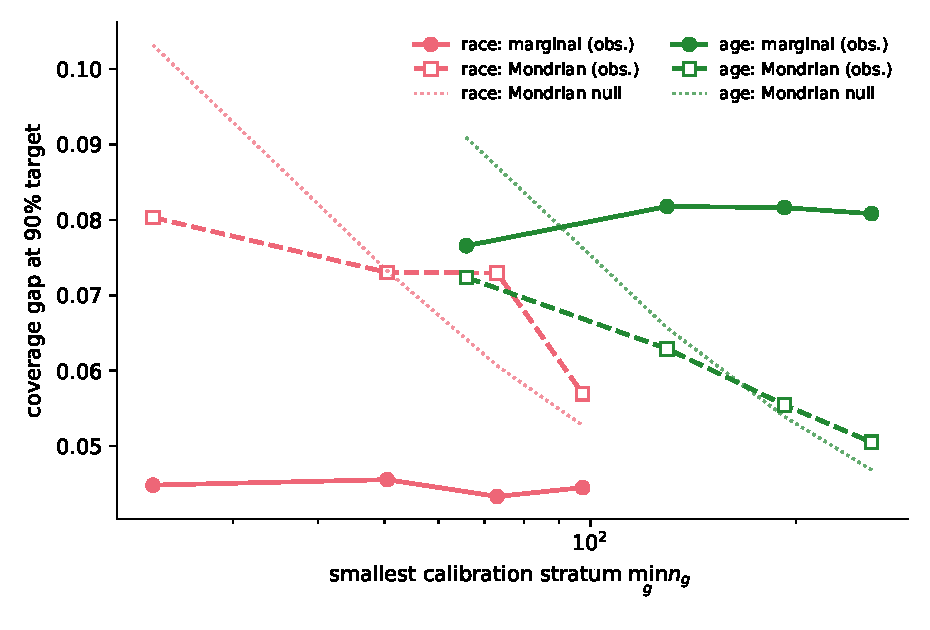
\includegraphics[width=0.78\linewidth]{gap_vs_support}
\caption{Coverage gap at the $90\%$ target versus the smallest calibration stratum $\min_g n_g$, obtained by subsampling each model's calibration set to $n_{\mathrm{cal}}\in\{500,1000,1500,2000\}$ (LAC; pooled over the four base models, datasets, seeds). Solid: marginal (observed); dashed: Mondrian (observed); dotted: simulated zero-bias Mondrian null. Race (red): Mondrian stays above marginal and worsens as support shrinks. Age (green): Mondrian repairs the marginal bias, and the repair weakens toward small support. Observed Mondrian gaps track their nulls throughout.}
\label{fig:sweep}
\end{figure}

\subsection{The efficiency cost of equalized coverage: a set-size tax}
\label{sec:rq3tax}
Coverage equity is only half of fairness for prediction sets; the other half is whether the \emph{size} of those sets---the amount of irreducible uncertainty each group is told it faces---is distributed evenly. Table~\ref{tab:tax} reports the set-size disparity $\max_g \bar k_g - \min_g \bar k_g$ at the $90\%$ target under LAC: \emph{Mondrian calibration improves coverage equity at the expense of efficiency equity}. On the age axis, where Mondrian nearly halves the coverage gap, it simultaneously raises the set-size disparity from $0.240$ to $0.373$---a $55\%$ increase. The same direction holds on every axis (sex $0.059\!\to\!0.086$; race $0.118\!\to\!0.154$; predicted class $0.115\!\to\!0.160$): equalizing coverage forces the harder-to-cover groups to carry visibly larger sets. The effect is mechanical---restoring a group's coverage to nominal when its scores are less separable requires admitting more labels---and there is a legitimate normative reading on which it is \emph{desirable}: Romano et al.\ \cite{romano2020eq} argue that larger sets for harder groups are the honest expression of genuinely higher uncertainty, preferable to quiet under-coverage. We do not adjudicate that question; our point is narrower and operational. The two disparities are distinct, they move in opposite directions under stratification, and a practitioner who monitors only the coverage gap will not see the set-size redistribution at all. Both should be reported, and which harm to prioritize---an omitted true label or an inflated ``maybe''---is a domain decision, not a statistical one.

\begin{table}[t]
\centering
\caption{RQ3 --- Set-size disparity $\max_g \bar k_g - \min_g \bar k_g$ at the $90\%$ target (LAC; pooled over base models and cells). Mondrian calibration lowers the coverage gap (Table~\ref{tab:rq3}) but raises the set-size disparity on every axis.}
\label{tab:tax}
\small
\begin{tabular}{lcccc}
\toprule
Method & Sex & Age & Race & Pred.\ class \\
\midrule
Marginal & $0.059$ & $0.240$ & $0.118$ & $0.115$ \\
Mondrian & $0.086$ & $0.373$ & $0.154$ & $0.160$ \\
\bottomrule
\end{tabular}
\end{table}

\begin{figure}[t]
\centering

\includegraphics[width=0.85\linewidth]{coverage_gap_age}
\caption{Coverage gap by age at the $90\%$ target, marginal vs.\ Mondrian, per base model (LAC score). Mondrian reduces the gap by roughly $0.03$ uniformly across models. Bars are per-model means; error bars are the standard deviation over the $15$ (dataset $\times$ seed) cells, and the $y$-axis range is shared across Figs.~\ref{fig:gapage}--\ref{fig:gaprace}.}
\label{fig:gapage}
\end{figure}

\begin{figure}[t]
\centering

\includegraphics[width=0.85\linewidth]{coverage_gap_sex}
\caption{Coverage gap by sex at the $90\%$ target (LAC score), per base model; bars and error bars as in Fig.~\ref{fig:gapage}. Gaps are an order of magnitude smaller than on age and statistically indistinguishable between methods.}
\label{fig:gapsex}
\end{figure}

\begin{figure}[t]
\centering

\includegraphics[width=0.85\linewidth]{coverage_gap_race}
\caption{Coverage gap by race at the $90\%$ target (LAC score), per base model; bars and error bars as in Fig.~\ref{fig:gapage}. Mondrian exceeds marginal for every model: with small calibration strata, group-conditional thresholds are noisy and realized disparities grow---matching the simulated null of Table~\ref{tab:mcnull}.}
\label{fig:gaprace}
\end{figure}

% =====================================================================
\section{Discussion}
\label{sec:discussion}

\paragraph{What the audit establishes about TabPFN.}
Within the studied regime---binary census tasks, moderate sample sizes, five seeds---TabPFN's uncertainty is trustworthy on the first two criteria of Section~\ref{sec:intro}: its native probabilities are as well calibrated as anything we tested without post-processing, and they translate into the most efficient conformal sets. Both findings are consistent with the PFN design: a model meta-trained to approximate a posterior predictive should produce probabilities whose ordering and sharpness reflect genuine predictive uncertainty, and LAC efficiency is exactly a function of probability quality. The practical upshot---pending the recalibrated-GBDT comparison of Table~\ref{tab:rq1}---is that the usual deployment recipe for boosted trees (train, then recalibrate) can be dropped for TabPFN in this regime; temperature scaling moved pooled ECE by one point in the third decimal.

\paragraph{What it establishes about conformal fairness.}
The third criterion---equitable uncertainty---is not a model property at all in our data. Coverage gaps under marginal calibration are nearly identical across predictors, and so is the effect of Mondrian stratification. The decision that matters is procedural: \emph{which taxonomy to condition on, given its calibration support}. Our results give a clean demonstration of both sides: conditioning on age (few, large groups, with a real disparity to fix) nearly halves the gap at the cost of $0.02$ extra labels per set; conditioning on race (a very small stratum, little demonstrated bias) backfires, inflating realized disparity without improving the worst group. This is not a contradiction of the equalized-coverage guarantee, which is an expectation over calibration randomness; it is the finite-sample variance of that guarantee made visible---and made \emph{predictable}.

\paragraph{A diagnostic, not just a diagnosis.}
The null model of Section~\ref{sec:theory} turns the race-axis failure from an anomaly into a checkable precondition. Before conditioning on any axis, a practitioner should (1) simulate the zero-bias marginal null and the Mondrian null from $\{\alpha, \{n_g\}, \{m_g\}\}$---seconds of computation with the committed script---and (2) compare the observed marginal gap to both. If the marginal gap does not clearly exceed the zero-bias null, no structural bias has been demonstrated and stratification is unjustified; if it exceeds the zero-bias null but not the Mondrian null, there is bias, but stratification would replace it with at least as much noise---prefer merging strata or methods with explicit small-sample control \cite{gibbs2023,jung2023,ding2023,lofstrom2015}; only if it exceeds both is plain Mondrian calibration expected to help. The closed form of Eq.~\eqref{eq:gapfloor} gives the scaling ($1/\sqrt{\min_g n_g}$, $\sqrt{\ln|\mathcal{G}|}$) for back-of-envelope use; as a coarse corollary, a stratum needs on the order of $n_g \gtrsim 10/\alpha$ points before its threshold is stable enough to be worth estimating separately, and our axes straddle exactly this line (age 65+: $n_g = 140$ at $\alpha=0.1$, helped; race Black: $n_g = 84$, harmed). This reframes ``equalized coverage'' from an unconditional good into a decision with a computable precondition---a stance in the approximate-reasoning tradition of asking \emph{when} a guarantee is informative.

\paragraph{Deployment guidance.}
For practitioners deploying small-to-medium tabular classifiers with demographic structure, our results support the following sequence. (1) If TabPFN's scale limits permit, it is a strong default: best accuracy and proper scores in our tests, no recalibration step. (2) Wrap the model in split conformal prediction with the LAC score; if APS is preferred for its adaptivity, verify that the implementation randomizes before using it on low-cardinality label spaces, and monitor empty-set rates under LAC. (3) Before choosing between marginal and Mondrian calibration on an axis, run the null-model diagnostic above. (4) Report worst-group coverage and named per-group coverage alongside marginal coverage---the latter alone certified all our models while one age group received $73\%$ coverage at an $80\%$ target---and report the set-size disparity alongside the coverage gap, since the two move in opposite directions under stratification.

\paragraph{TabPFN versus GBDTs, scoped.}
Our comparison favours TabPFN on every uncertainty metric, with three caveats that bound the claim. The tasks sit squarely inside TabPFN's comfort zone ($3{,}600$ training rows per cell, census features, binary labels); the GBDTs received no hyperparameter tuning, and a tuning budget would likely close part of the gap (the temperature-scaled rows of Table~\ref{tab:rq1} quantify how much of it recalibration alone recovers); and GBDT inference is orders of magnitude cheaper at scale. Where these constraints bind, the correct reading is narrower but still useful: GBDT probabilities should not be consumed raw, and conformal wrapping equalizes validity---though not efficiency---across model families.

% =====================================================================
\section{Limitations and threats to validity}
\label{sec:limitations}

\emph{External validity.} All results derive from three binary tasks on Californian ACS microdata from a single survey year; the three tasks share respondents and feature space, so they are closer to one population with three label definitions than to independent datasets. Conclusions are scoped to this regime and should not be extrapolated to multiclass problems, other states or years, non-census domains, or tables beyond TabPFN's supported size. Replication across a second state (e.g.\ Texas), which would vary the demographic profile and the $n_g$ structure, is left to future work; our pipeline parameterizes the state, so this is a configuration change rather than a methodological extension. We did, however, run the natural further stress of the noise floor---an intersectional sex\,$\times$\,race taxonomy of up to eight strata, the smallest holding only $\approx\!34$ calibration points: its marginal gap at the $90\%$ target is $0.082$ and Mondrian stratification \emph{increases} it to $0.099$ ($n=15$, $p=0.013$), a sharper instance of the same small-group failure, exactly as the floor predicts for smaller $\min_g n_g$ and larger $|\mathcal{G}|$. \emph{Designed regime.} The small-group regime is induced by our subsampling (Section~\ref{sec:designed}); on the full ACS data the calibration set could be enlarged until every stratum clears the floor. \emph{Construct validity.} ECE estimates depend on binning; we mitigate with adaptive binning and proper scoring rules, which agree in direction. The max--min coverage gap is group-count sensitive and anonymous; we mitigate by reporting worst-group coverage, named per-group coverage, and---centrally---by reading every gap against its finite-sample null rather than against zero. The four-way race coarsening is an analytic choice; finer partitions shrink $\min_g n_g$ and raise the floor, so our race-axis conclusions are conservative in that direction but sensitive to the merging of heterogeneous categories into ``Other''. \emph{Internal validity.} Baseline hyperparameters were fixed at common defaults with no per-dataset tuning; the temperature-scaled GBDT rows isolate the recalibration component of that budget, but a fuller tuning study could narrow the remaining gaps. Five seeds bound our resolution. \emph{Statistical validity.} Wilcoxon tests at $n=15$ have a floor of $p=6.1\times10^{-5}$; RQ3 contrasts are paired at the model-averaged (dataset $\times$ seed) level with Holm adjustment (Section~\ref{sec:stats}); Friedman ranks are descriptive. We did not run distribution-shift experiments, so exchangeability holds by construction here and coverage under shift is untested. \emph{Theoretical scope.} The null model of Section~\ref{sec:theory} is exact for the zero-bias case given continuous scores, independent strata, and the stated group sizes; the closed form of Eq.~\eqref{eq:gapfloor} is a heuristic whose accuracy region we characterize empirically (Fig.~\ref{fig:mcnull}). A rigorous finite-sample bound on the gap statistic under nonzero bias, and an analysis of dependence induced by shared score functions, are left to future work. \emph{Model specificity.} The audited model is one public checkpoint (TabPFN v3, \texttt{tabpfn-v3-classifier-v3\_default.ckpt}); conclusions about ``TabPFN'' are conclusions about that release. \emph{Ethical scope.} Equalizing coverage is one narrow fairness criterion; it neither implies nor substitutes for fairness of the underlying decisions, and the race categories in ACS data are coarse administrative constructs whose coarsening we performed further.

% =====================================================================
\section{Conclusion and future work}
\label{sec:conclusion}

We showed that marginal conformal validity is not subgroup validity, and---more usefully---that the gap between them can be \emph{predicted} before any group-conditional calibration is run. Across multiple predictors and three census tasks, split conformal prediction met its marginal guarantee while concealing an eight-point age coverage gap common to all models; group-conditional (Mondrian) calibration repaired this where strata were large but backfired on the small-support race axis. An exact, simulable zero-bias null---built from the Beta law of split-conformal coverage and a binomial measurement layer, requiring only $\{\alpha, \{n_g\}, \{m_g\}\}$---decomposed every observed gap into structural bias and sampling noise, predicted the sign of the marginal-to-Mondrian change on every axis, and matched the post-stratification gaps to within $0.005$ at the primary target. These effects were governed by the conformal procedure and the group structure rather than the model. As the audited model, TabPFN proved the most reliable base learner we tested: natively well calibrated, requiring no temperature scaling, and yielding the smallest conformal sets at every level---within the regime and configurations studied. We also documented, as a deployment caution, the silent total degeneracy of non-randomized APS on binary tasks.

Future work proceeds on four fronts. (i) Populating the $(\min_g n_g,\,|\mathcal{G}|)$ plane with more group structures---additional states and an OpenML extension---to stress-test the null model where it is least accurate (many comparably small strata). (ii) Distribution-shift stress tests---cross-state and temporal transfer within ACS---probing coverage and calibration degradation when exchangeability fails \cite{ovadia2019}, with adaptive remedies \cite{gibbs2021,tibshirani2019}. (iii) A multiclass study re-opening the APS question, where randomized and label-shared variants \cite{romano2020aps,angelopoulos2021,ding2023} should behave very differently, and where risk-controlling generalizations of coverage \cite{bates2021} offer alternative targets. (iv) A clinical-tabular extension, where small protected strata are unavoidable rather than designed, making the noise-floor diagnostic the central methodological tool rather than a robustness check.

Beyond the specific findings, the paper argues for a reporting norm: an in-expectation guarantee should be published together with the finite-sample null under which it is informative. For group-conditional conformal prediction that null is exactly computable in seconds, model-free, and validated here on three protected axes; analogous nulls should govern other group-conditional procedures (class-conditional conformal prediction, multivalid calibration, group-wise recalibration) wherever a guarantee is bought with per-group data. Making that purchase price explicit is, we argue, the right default for deploying set-valued predictors in consequential, demographically structured settings.

% =====================================================================
\section*{Reproducibility statement}
All code, notebooks, the complete per-seed result files (\texttt{calibration.csv}; \texttt{conformal\_fairness.csv}), the null-model simulator (\texttt{scripts/mc\_noise\_floor.py}; 200{,}000 replicates, seconds on CPU), the re-pairing analysis script (\texttt{scripts/repaired\_stats.py}), and the prediction-cache and derivation scripts (\texttt{scripts/build\_cache.py}, \texttt{scripts/derive\_from\_cache.py}, which produce the per-group, empty-set, randomized-APS, and recalibrated-GBDT results) are released at \url{https://github.com/Nadim-Mahmud-23/tabpfn-uncertainty-audit} under the MIT license, with pinned dependency versions: \texttt{tabpfn} 8.0.7 (PyTorch 2.9.1 backend, checkpoint \texttt{tabpfn-v3-classifier-v3\_default.ckpt}), \texttt{xgboost} 3.2.0, \texttt{lightgbm} 4.6.0, \texttt{scikit-learn} 1.8.0, \texttt{folktables} 0.0.12, \texttt{numpy} 2.3.5, and \texttt{scipy} 1.17.0 under Python 3.11+. Every table and statistic is regenerable from the committed CSVs by the analysis scripts; figures regenerate from the same files; an archival copy of the result files and analysis scripts is deposited at Zenodo (\url{https://doi.org/10.5281/zenodo.20662098}). Data are downloaded automatically from the US Census Bureau via folktables. All experiments run on a single Apple Silicon MacBook with no GPU; the committed experiment matrix completes in approximately one hour of wall-clock time, dominated by TabPFN's CPU inference.

\section*{Funding}
No funding was received for this research.

\section*{Declaration of competing interest}
The author declares that he has no known competing financial interests or personal relationships that could have appeared to influence the work reported in this paper.

\section*{CRediT authorship contribution statement}
\textbf{Nadim Mahmud Dipu:} Conceptualization, Methodology, Software, Validation, Formal analysis, Investigation, Data curation, Writing -- original draft, Writing -- review \& editing, Visualization.

\section*{Data availability}
The data used in this study are publicly available from the U.S.\ Census Bureau American Community Survey (ACS) Public Use Microdata Sample (PUMS), 2018 1-Year release, accessed programmatically via the folktables package \cite{ding2021}. All source code, notebooks, and the committed per-seed result files needed to reproduce every table and figure are released in the repository cited in the Reproducibility statement.

\section*{Declaration of generative AI and AI-assisted technologies in the writing process}
During the preparation of this work the author used Claude (Anthropic), an AI assistant, to support the drafting and editing of the manuscript text. After using this tool, the author reviewed and edited the content as needed and takes full responsibility for the content of the publication.

% =====================================================================
\bibliographystyle{elsarticle-num}
\bibliography{refs}

\end{document}
